\apendice{Especificación de Requisitos}\label{anex:B}

\section{Introducción}

En este anexo se analizan y documentan las diferentes necesidades funcionales y no funcionales que deberán ser soportadas por la aplicación generada en este proyecto. Se van a nombrar tanto los requisitos del proyecto original\cite{TFGPrevio} como los del proyecto actual pues éste último ha de cumplir ambos.


\section{Objetivos generales}
El objetivo general de este TFG es mantener la funcionalidad implementada en el proyecto original\cite{TFGPrevio} y mejorarla incluyendo nuevas métricas y realizando la integración con \textit{GitHub}para poder trabajar con repositorios alojados allí. Además se implementarán mejoras de la interfaz para mejorar la usabilidad y se corregirán errores.

Por tanto se pueden nombrar los siguientes objetivos:
\begin{itemize}
	\tightlist
	\item Se obtendrán medidas de métricas de evolución de uno o varios proyectos alojados en repositorios tanto en \textit{GitLab} como en \textit{GitHub}.
	\item Las métricas que se desean calcular de un repositorio  son algunas de las especificadas en la tesis titulada ``\textit{sPACE: Software Project Assessment in the Course of Evolution}'' \cite{ratzinger_space:_2007} y 
	adaptadas a los repositorios software junto a nuevas métricas relacionadas con la integración y despliegue continuos (las 5 últimas):
	\begin{itemize}
		\tightlist
		\item Número total de incidencias (\textit{issues})
		\item Cambios (\textit{commits}) por incidencia
		\item Porcentaje de incidencias cerrados
		\item Media de días en cerrar una incidencia
		\item Media de días entre cambios
		\item Días entre primer y último cambio
		\item Rango de actividad de cambios por mes
		\item Porcentaje de pico de cambios
		\item Número total de \textit{jobs} ejecutados
		\item Número de \textit{jobs} ejecutados el último año
		\item Número de tipos diferentes de \textit{jobs} ejecutados
		\item Número total de \textit{releases}
		\item Número de \textit{releases} lanzadas el último año
		
	\end{itemize}
	\item Se pretende ser capaces de evaluar el estado de un proyecto comparándolo con otros proyectos por medio del uso de las métricas anteriores. Para ello se deberán establecer unos valores umbrales por cada métrica basados en el cálculo de los cuartiles Q1 y Q3.\\
	 Además, estos valores se podrán calcular dinámicamente y se almacenarán en perfiles de configuración de métricas. Estos umbrales deberán existir para todas la métricas, incluidas las nuevas.
	\item Se dará la posibilidad de almacenar de manera persistente estos perfiles de métricas para permitir comparaciones futuras. 
	\item También se permitirá almacenar de forma persistente las métricas obtenidas de los repositorios para su posterior consulta o tratamiento. Esto permitiría comparar nuevos proyectos con proyectos de los que ya se han calculado sus métricas.
	\item La persistencia debe incluir también las nuevas métricas, tanto para la exportación como para la importación de los valores de las mismas.
\end{itemize}

\section{Objetivos técnicos}
Este apartado resume requisitos del proyecto más técnicos y centrados en el proceso y otras características no funcionales.
\begin{itemize}
	\tightlist
	\item Utilizar el diseño basado en \textit{frameworks}  y en patrones de diseño \cite{gamma_patrones_2002} existente para implementar las nuevas métricas.
	\item Utilizar y adaptar en lo necesario el diseño de la aplicación para extender a \textit{GitHub}su funcionalidad y seguir permitiendo la extensión otras plataformas de desarrollo colaborativo como \textit{Bitbucket}.
	\item Crear una batería de pruebas automáticas en los subsistemas de lógica de la aplicación.
	\item Utilizar una plataforma de desarrollo colaborativo que incluya un sistema de control de versiones, un sistema de seguimiento de incidencias y que permita una comunicación fluida entre el tutor y el alumno. Se sugiere la utilización de \textit{GitHub}.
	\item Utilizar un sistema de integración y despliegue continuo.
	\item Mejorar la gestión de errores existente tratando excepciones de biblioteca y de la propia aplicación y registrar dichos eventos de error e información en ficheros de \textit{log}. 
	\item Probar la aplicación con ejemplos reales y utilizando técnicas avanzadas, como entrada de datos de test en ficheros con formato tabulado tipo CSV (\textit{Comma Separated Values}). 	
\end{itemize}

\section{Actores}
Se consideran dos actores:
\begin{itemize}
	\tightlist
	\item El usuario de la aplicación, es aquella persona que utilice la aplicación.
	\item El desarrollador, que a su vez puede ser considerado como usuario pero que además tiene las labores de implementación y mantenimiento de la aplicación.
\end{itemize}

\section{Catálogo de requisitos}
En esta sección se van a enumerar los requisitos que el sistema tendrá que satisfacer. Están divididos en dos tipos, en el primero se basa en funcionalidad y el segundo en aspectos del proceso de desarrollo y aspectos técnicos del sistema como la mantenibilidad.

\subsection{Requisitos funcionales}

\begin{itemize}
\item \textbf{RF-1} Establecer conexión con \textit{GitHub}: El usuario debe poder establecer conexión con \textit{GitHub}.
	\begin{itemize}
		\item \textbf{RF-1.1} Debido a las restriccones que tiene la \textit{API} de \textit{GitHub} y que se \textit{deprecó} el acceso del usuario por usuario y contraseña\footnote{Autenticación en \textit{GitHub API} - \url{https://docs.github.com/es/rest/overview/other-authentication-methods}}, el usuario podrá iniciar sesión desde la aplicación sólo mediante un token de acceso personal a su usuario en \textit{GitHub}para poder obtener los repositorios públicos y privados a los que tenga acceso.
		\item \textbf{RF-1.2} La aplicación mostrará al usuario en todo momento la conexión que está utilizando
		\item \textbf{RF-1.3} El usuario podrá utilizar la aplicación sin establecer una conexión. Aunque no tenga acceso a los repositorios de \textit{GitHub}.
		\item \textbf{RF-1.4} El usuario podrá cambiar de conexión teniendo en cuenta que sólo puede haber un tipo de conexión con \textit{GitHub} activo en un instante dado. Esta conexión será independiente de la posible conexión con \textit{GitLab}.

	\end{itemize}
	\item \textbf{RF-2} Establecer conexión con \textit{GitLab}: El usuario debe poder establecer distintos tipos de conexión a \textit{GitLab}.
	\begin{itemize}
		\item \textbf{RF-2.1} El usuario podrá iniciar sesión desde la aplicación mediante usuario y contraseña a su usuario en \textit{GitLab} para poder obtener los repositorios públicos y privados a los que tenga acceso.
		\item \textbf{RF-2.2} El usuario podrá iniciar sesión desde la aplicación mediante un token de acceso personal a su usuario en \textit{GitLab} para poder obtener los repositorios públicos y privados a los que tenga acceso.
		\item \textbf{RF-2.3} El usuario podrá establecer una conexión pública a \textit{GitLab} para poder obtener los repositorios públicos.
		\item \textbf{RF-2.4} El usuario podrá utilizar la aplicación sin establecer una conexión. Aunque no tenga acceso a los repositorios de \textit{GitLab}.
		\item \textbf{RF-2.5} El usuario deberá elegir un tipo de conexión al entrar por primera vez a la aplicación.
		\item \textbf{RF-2.6} La aplicación mostrará al usuario en todo momento la conexión que está utilizando
		\item \textbf{RF-2.7} El usuario podrá cambiar de conexión teniendo en cuenta que sólo puede haber un tipo de conexión con \textit{GitLab} activo en un instante dado. Esta conexión será independiente de la posible conexión con \textit{GitHub}.
	\end{itemize}
	\item \textbf{RF-3} Gestión de proyectos. El usuario podrá calcular las métricas de proyectos tanto de \textit{GitHub}como de \textit{GitLab} definidas en la sección \ref{sect:B_5_1_1}: `\textit{Definición de las métricas}' y se mostrarán los resultados en forma de tabla en la que las filas se correspondan con los proyectos y las columnas con las métricas.
	\begin{itemize}
		\item \textbf{RF-3.1} El usuario podrá añadir un proyecto siempre que tenga una conexión a \textit{GitLab} o con \textit{GitHub} (dependiendo del dónde esté alojado dicho proyecto):
		\begin{itemize}
			\item \textbf{RF-3.1.1} El usuario podrá añadir un proyecto a partir del nombre de usuario o ID del propietario y el nombre del proyecto, siempre que tenga acceso desde la conexión establecida.
			\item \textbf{RF-3.1.2} El usuario podrá añadir un proyecto a partir del nombre o del ID del grupo al que pertenece el proyecto y su nombre, siempre que tenga acceso desde la conexión establecida.
			\item \textbf{RF-3.1.3} El usuario podrá añadir un proyecto a partir de su URL, siempre que tenga acceso desde la conexión establecida.
		\end{itemize}
		\item \textbf{RF-3.2} El usuario no podrá añadir un proyecto que ya esté en la tabla.
		\item \textbf{RF-3.3} Al añadir un proyecto a la tabla se calcularán las métricas definidas en la sección \ref{sect:B_5_1_1}: `\textit{Definición de las métricas}' y se mostrarán en forma de tabla.
		\item \textbf{RF-3.4} El usuario podrá eliminar un proyecto de la tabla.
		\item \textbf{RF-3.5} El usuario podrá volver a obtener las métricas de un repositorio que ya haya añadido, siempre que tenga acceso desde la conexión establecida (con \textit{GitHub}o \textit{GitLab} dependiendo de dónde esté alojado el proyecto).
		\item \textbf{RF-3.6} El usuario podrá exportar los proyectos y sus métricas a un fichero con formato `\ruta{.emr}'.
		\item \textbf{RF-3.7} El usuario podrá exportar los resultados de las métricas de todos los proyectos en un fichero con formato CSV.
		\item \textbf{RF-3.8} El usuario podrá importar y añadir repositorios a la tabla  desde un fichero con formato `\ruta{.emr}', respetando el requisito RF3.2 de no añadir un repositorio ya existente.
		\item \textbf{RF-3.9} El usuario podrá importar repositorios a la tabla, sobrescribiendo los de la tabla.
		\item \textbf{RF-3.10} Se podrán filtrar los proyectos por su nombre.
		\item \textbf{RF-3.11} Se puede ordenar los repositorios por nombre, fecha de medición y por cualquiera de las métricas.
		\item \textbf{RF-3.12} Al ordenar por las nuevas métricas relacionadas con \textit{CICD} habrá que tener en cuenta que habrá medidas que no se habrán calculado por falta de datos de \textit{GitLab} si no se ha realizado conexión \textit{autenticada} pues \textit{GitLab API} no devuelve información  sobre \textit{jobs} y \textit{releases} con conexión pública.
	\end{itemize}
	\item \textbf{RF-4} Evaluación de métricas. Las métricas, una vez calculadas, serán evaluadas mediante un código de color (verde - bueno, naranja - peligro, rojo - malo) a partir de un perfil de métricas, que será un conjunto de valores mínimo y máximo de cada una de las métricas, a partir de la definición de la evaluación en la sección \ref{sect:B_5_1_2}: `\textit{Evaluación de métricas}'. Esto ha de aplicarse también a las nuevas métricas que se implementen no sólo a las existentes.
	\begin{itemize}
		\item \textbf{RF-4.1} Se podrá cargar un perfil de métricas que contenga valores umbrales mínimo y máximo y se utilizarán para evaluarlas.
		\item \textbf{RF-4.2} El usuario podrá cargar un perfil por defecto creado a partir de un conjunto de datos \footnote{\url{https://github.com/clopezno/clopezno.github.io/blob/master/agile_practices_experiment/DataSet_EvolutionSoftwareMetrics_FYP.csv}} de un estudio empírico de las métricas de evolución del software en trabajos finales de grado\cite{lopez_nozal_measuring_2019}.
		\item \textbf{RF-4.3} El usuario podrá cargar un perfil creado a partir de los repositorios que existan en la tabla.
		\item \textbf{RF-4.4} El usuario podrá exportar el perfil de métricas que tenga cargado a un fichero con formato \ruta{emmp}.
		\item \textbf{RF-4.5} El usuario podrá importar un perfil de métricas que haya guardado anteriormente para evaluar los repositorios que tenga en la tabla.
		\item \textbf{RF-4.6} En un instante, sólo puede haber un perfil de métricas cargado.
		\item \textbf{RF-4.7} Al inicio se cargará el perfil de evaluación por defecto.
	\end{itemize}
\end{itemize}

\subsubsection{Definición de las métricas}\label{sect:B_5_1_1}

En el requisito RF-3 implica que se deben calcular las siguientes métricas de un proyecto:

\textbf{\underline{I1 - Número total de \textit{issues} (incidencias)}}

\begin{itemize}
	\item \textbf{Categoría}: Proceso de Orientación
	\item \textbf{Descripción}: Número total de \textit{issues} creadas en el repositorio
	\item \textbf{Propósito}: ¿Cuántas \textit{issues} se han definido en el repositorio?
	\item \textbf{Fórmula}: $NTI$. \textit{NTI = número total de \textit{issues}}
	\item \textbf{Fuente de medición}: Proyecto en una plataforma de desarrollo colaborativo.
	\item \textbf{Interpretación}: $NTI \geq 0$. Valores bajos indican que no se utiliza un sistema de seguimiento de incidencias, podría ser porque el proyecto acaba de comenzar
	\item \textbf{Tipo de escala}: Absoluta
	\item \textbf{Tipo de medida}: \textit{NTI = Contador}
\end{itemize}

\textbf{\underline{I2 - \textit{Commits} (cambios) por \textit{issue}}}

\begin{itemize}
	\item \textbf{Categoría}: Proceso de Orientación
	\item \textbf{Descripción}: Número de \textit{commits} por \textit{issue}
	\item \textbf{Propósito}: ¿Cuál es el volumen medio de trabajo de las \textit{issues}?
	\item \textbf{Fórmula}: $CI = \frac{NTC}{NTI}$. \textit{CI = Cambios por \textit{issue}, NTC = Número total de \textit{commits}, NTI = \textbf{Número} total de \textit{issues}}
	\item \textbf{Fuente de medición}: Proyecto en una plataforma de desarrollo colaborativo.
	\item \textbf{Interpretación}: $CI \geq 1$, Lo normal son valores altos. Si el valor es menor que uno significa que hay desarrollo sin documentar.
	\item \textbf{Tipo de escala}: Ratio 
	\item \textbf{Tipo de medida}: \textit{NTC, NTI = Contador}
\end{itemize}

\textbf{\underline{I3 - Porcentaje de \textit{issues} cerradas}}

\begin{itemize}
	\item \textbf{Categoría}: Proceso de Orientación
	\item \textbf{Descripción}: Porcentaje de \textit{issues} cerradas
	\item \textbf{Propósito}: ¿Qué porcentaje de \textit{issues} definidas en el repositorio se han cerrado?
	\item \textbf{Fórmula}: $PIC = \frac{NTIC}{NTI}*100$. \textit{PIC = Porcentaje de \textit{issues} cerradas, NTIC = Número total de \textit{issues} cerradas, NTI = Número total de \textit{issues}}
	\item \textbf{Fuente de medición}: Proyecto en una plataforma de desarrollo colaborativo.
	\item \textbf{Interpretación}: $0 \leq PIC \leq 100$. Cuanto más alto mejor
	\item \textbf{Tipo de escala}: Ratio
	\item \textbf{Tipo de medida}: \textit{NTI, NTIC = Contador}
\end{itemize}

\textbf{\underline{TI1 - Media de días en cerrar una \textit{issue}}}

\begin{itemize}
	\item \textbf{Categoría}: Constantes de tiempo
	\item \textbf{Descripción}:  Media de días en cerrar una \textit{issue}
	\item \textbf{Propósito}: ¿Cuánto se suele tardar en cerrar una \textit{issue}? 
	\item \textbf{Fórmula}: $MDCI = \frac{\sum_{i=0}^{NTIC}DCI_i}{NTIC}$. \textit{MDCI = Media de días en cerrar una \textit{issue}, NTIC = Número total de \textit{issues} cerradas, DCI = Días en cerrar la \textit{issue}}
	\item \textbf{Fuente de medición}: Proyecto en una plataforma de desarrollo colaborativo.
	\item \textbf{Interpretación}: $MDCI \geq 0$. Cuanto más pequeño mejor. Si se siguen metodologías ágiles de desarrollo iterativo e incremental como \textit{SCRUM}, la métrica debería indicar la duración del \textit{sprint} definido en la fase de planificación del proyecto. En \textit{SCRUM} se recomiendan duraciones del \textit{sprint} de entre una y seis semanas, siendo recomendable que no exceda de un mes \cite{scrum_master_scrum_2019}.
	\item \textbf{Tipo de escala}: Ratio
	\item \textbf{Tipo de medida}: \textit{NTI, NTIC = Contador}
\end{itemize}

\textbf{\underline{TC1 - Media de días entre \textit{commits}}}

\begin{itemize}
	\item \textbf{Categoría}: Constantes de tiempo
	\item \textbf{Descripción}: Media de días que pasan entre dos \textit{commits} consecutivos
	\item \textbf{Propósito}: ¿Cuántos días suelen pasar desde un \textit{commit} hasta el siguiente?
	\item \textbf{Fórmula}: $MDC = \frac{\sum_{i=1}^{NTC} TC_i - TC_{i-1}}{NTC}$. $TC_i - TC_{i-1}$ en días; \textit{MDC = Media de días entre cambios, NTC = Número total de \textit{commits}, TC = Tiempo de \textit{commit}}
	%$MDEC = [Sumatorio de (TCi-TCj) desde i=1, j=0 hasta i=NTC] / NTC. NTC = Número total de \textit{commits}, TC = Tiempo de Commit$ 
	\item \textbf{Fuente de medición}: Proyecto en una plataforma de desarrollo colaborativo.
	\item \textbf{Interpretación}: $MDEC \geq 0$. Cuanto más pequeño mejor. Se recomienda no superar los 5 días.
	\item \textbf{Tipo de escala}: Ratio
	\item \textbf{Tipo de medida}: \textit{NTC = Contador; TC = Tiempo}
\end{itemize}

\textbf{\underline{TC2 - Días entre primer y último \textit{commit}}}

\begin{itemize}
	\item \textbf{Categoría}: Constantes de tiempo
	\item \textbf{Descripción}: Días transcurridos entre el primer y el último \textit{commit} 
	\item \textbf{Propósito}: ¿Cuántos días han pasado entre el primer y el último \textit{commit}?
	\item \textbf{Fórmula}: $DEPUC = TC2- TC1$. $TC2- TC1$ en días;  \textit{DEPUC = Días entre primer y último \textit{commit}, TC2 = Tiempo de último \textit{commit}, TC1 = Tiempo de primer \textit{commit}}
	\item \textbf{Fuente de medición}: Proyecto en una plataforma de desarrollo colaborativo.
	\item \textbf{Interpretación}: $DEPUC \geq 0$. Cuanto más alto, más tiempo lleva en desarrollo el proyecto. En procesos software empresariales se debería comparar con la estimación temporal de la fase de planificación. 
	\item \textbf{Tipo de escala}: Absoluta
	\item \textbf{Tipo de medida}: \textit{TC = Tiempo}
\end{itemize}

\textbf{\underline{TC3 - Ratio de actividad de \textit{commits} por mes}}

\begin{itemize}
	\item \textbf{Categoría}: Constantes de tiempo
	\item \textbf{Descripción}: Muestra el número de \textit{commits} relativos al número de meses
	\item \textbf{Propósito}:¿Cuál es el número medio de cambios por mes?
	\item \textbf{Fórmula}: $RCM = \frac{NTC}{NM}$. \textit{RCM = Ratio de cambios por mes, NTC = Número total de \textit{commits}, NM = Número de meses que han pasado durante el desarrollo de la aplicación}
	\item \textbf{Fuente de medición}: Proyecto en una plataforma de desarrollo colaborativo.
	\item \textbf{Interpretación}: $RCM > 0$. Cuanto más alto mejor
	\item \textbf{Tipo de escala}: Ratio
	\item \textbf{Tipo de medida}: \textit{NTC = Contador}
\end{itemize}

\textbf{\underline{C1 - Cambios pico}}

\begin{itemize}
	\item \textbf{Categoría}: Constantes de tiempo
	\item \textbf{Descripción}: Número de \textit{commits} en el mes que más \textit{commits} se han realizado en relación con el número total de \textit{commits}
	\item \textbf{Propósito}: ¿Cuál es la proporción de trabajo realizado en el mes con mayor número de cambios?
	\item \textbf{Fórmula}: $CP = \frac{NCMP}{NTC}$. \textit{CP = Cambios pico, NCMP = Número de \textit{commits} en el mes pico, NTC = Número total de \textit{commits}}
	\item \textbf{Fuente de medición}: Proyecto en una plataforma de desarrollo colaborativo.
	\item \textbf{Interpretación}: $0 \leq CCP \leq 1$. Mejor valores intermedios. Se recomienda no superar el 40\% del trabajo en un mes.
	\item \textbf{Tipo de escala}: Ratio
	\item \textbf{Tipo de medida}: \textit{NCMP, NTC = Contador}
\end{itemize}

\textbf{\underline{IC1 - Número total de \textit{jobs} ejecutados}}
\begin{itemize}
	\item \textbf{Categoría}: \textit{CICD}
	\item \textbf{Descripción}: Número de \textit{jobs} ejecutados en el proyecto.
	\item \textbf{Propósito}: ¿Cuál es el número total de de \textit{jobs} ejecutados con éxito en el proyecto?
	\item \textbf{Fórmula}: $NJE =$ \textit{número total de jobs}.
	\item \textbf{Fuente de medición}: Proyecto en una plataforma de desarrollo colaborativo.
	\item \textbf{Interpretación}: $NJE \geq 0$. Un valor de cero indica que el proyecto no tiene integración y despliegues continuos y no se ha realizado ningún trabajo automatizado de despliegue.
	\item \textbf{Tipo de escala}: Absoluta
	\item \textbf{Tipo de medida}: \textit{NJE = Contador}
\end{itemize}

\textbf{\underline{IC2 - Número de \textit{Jobs} ejecutados el último año}}
\begin{itemize}
	\item \textbf{Categoría}: \textit{CICD}
	\item \textbf{Descripción}: Número de \textit{jobs} ejecutados en el último año (últimos 365 días).
	\item \textbf{Propósito}: ¿Cuál es el número total de \textit{jobs} ejecutados con éxito en el proyecto durante el año previo?
	\item \textbf{Fórmula}: $NJELY =$ \textit{número total de jobs ejecutados el útimo año}.
	\item \textbf{Fuente de medición}: Proyecto en una plataforma de desarrollo colaborativo.
	\item \textbf{Interpretación}: $NJELY \geq 0$. Un valor de cero indica que en el proyecto no se ha realizado ningún trabajo automatizado de despliegue durante el último año.
	\item \textbf{Tipo de escala}: Absoluta
	\item \textbf{Tipo de medida}: \textit{NJELY = Contador}
\end{itemize}

\textbf{\underline{IC3 - \textit Número de tipos diferentes de{jobs} ejecutados}}
\begin{itemize}
	\item \textbf{Categoría}: \textit{CICD}
	\item \textbf{Descripción}: Número de tipos diferentes de \textit{jobs} ejecutados en el proyecto.
	\item \textbf{Propósito}: ¿Cuál es el número total de tipos de \textit{jobs} ejecutados con éxito en el proyecto?
	\item \textbf{Fórmula}: $NTJE =$ \textit{número total de tipos diferentes de jobs ejecutados en el proyecto}.
	\item \textbf{Fuente de medición}: Proyecto en una plataforma de desarrollo colaborativo.
	\item \textbf{Interpretación}: $NTJE \geq 0$. Un valor de cero indica que el proyecto no tiene integración y despliegues continuos y no se ha realizado ningún trabajo automatizado de despliegue.
	\item \textbf{Tipo de escala}: Absoluta
	\item \textbf{Tipo de medida}: \textit{NTJE = Contador}
\end{itemize}

\textbf{\underline{DC1 - \textit Número total de{releases}}}
\begin{itemize}
	\item \textbf{Categoría}: \textit{CICD}
	\item \textbf{Descripción}: Número de \textit{releases} lanzadas en el proyecto.
	\item \textbf{Propósito}: ¿Cuál es el número total de \textit{releases} del  proyecto?
	\item \textbf{Fórmula}: $NRR =$ \textit{número total de releases lanzadas en el proyecto}.
	\item \textbf{Fuente de medición}: Proyecto en una plataforma de desarrollo colaborativo.
	\item \textbf{Interpretación}: $NRR \geq 0$. Un valor de cero indica que aún no se ha lanzado ninguna \textit{release} del proyecto.
	\item \textbf{Tipo de escala}: Absoluta
	\item \textbf{Tipo de medida}: \textit{NRR = Contador}
\end{itemize}

\textbf{\underline{DC2 - \textit Número de{releases} lanzadas el último año}}
\begin{itemize}
	\item \textbf{Categoría}: \textit{CICD}
	\item \textbf{Descripción}: Número de \textit{releases} lanzadas en el proyecto en el último año (últimos 365 días).
	\item \textbf{Propósito}: ¿Cuál es el número total de \textit{releases} lanzadas en el proyecto durante el año previo?
	\item \textbf{Fórmula}: $NRRLY =$ \textit{número total de releases lanzadas en el proyecto en el último año}.
	\item \textbf{Fuente de medición}: Proyecto en una plataforma de desarrollo colaborativo.
	\item \textbf{Interpretación}: $NRRLY \geq 0$. Un valor de cero indica que no se ha lanzado ninguna \textit{release} del proyecto durante el último año.
	\item \textbf{Tipo de escala}: Absoluta
	\item \textbf{Tipo de medida}: \textit{NRRLY = Contador}
\end{itemize}

\subsubsection{Evaluación de métricas}\label{sect:B_5_1_2}
Las métricas se evaluarán como buenas si:
\begin{itemize}
	\item I1: El valor medido supera el umbral mínimo (Q1).
	\item I2: El valor medido se encuentra entre el umbral mínimo y el máximo (Q3).
	\item I3: El valor medido supera el umbral mínimo.
	\item TI1: El valor medido se encuentra entre el umbral mínimo y el máximo.
	\item TC1: El valor medido se encuentra entre el umbral mínimo y el máximo.
	\item TC2: El valor medido se encuentra entre el umbral mínimo y el máximo.
	\item TC3: El valor medido se encuentra entre el umbral mínimo y el máximo.
	\item C1: El valor medido se encuentra entre el umbral mínimo y el máximo.
	\item IC1: El valor medido supera el umbral mínimo. Si es el valor es 0 el proyecto no tiene integración y despliegue continuo.
	\item IC2: El valor medido supera el umbral mínimo. Si es el valor es 0 el proyecto no tiene integración y despliegue continuo.
	\item IC3: El valor medido supera el umbral mínimo. Si es el valor es 0 el proyecto no tiene integración y despliegue continuo.
	\item DC1: El valor medido supera el umbral mínimo. Si es el valor es 0 el proyecto aún no tiene ninguna \textit{release}.
	\item DC2: El valor medido supera el umbral mínimo.
\end{itemize}

\subsection{Requisitos no funcionales}

\begin{itemize}
	\item \textbf{RNF-1} Se debe mantener y mejorar el diseño extensible a otras forjas de repositorios para que tal y como se haga con \textit{GitHub}se pueda hacer en un futuro con otras forjas como \textit{Bitbucket}.
	\item \textbf{RNF-2} Se debe mantener y mejorar el diseño extensible y reutilizable a nuevas métricas, siguiendo el framework descrito en \textit{Soporte de Métricas con Independencia del Lenguaje para la Inferencia de Refactorizaciones} \cite{marticorena_sanchez_soporte_2005}.
	\item \textbf{RNF-3} El diseño de la interfaz ha de ser intuitivo y fácil de utilizar.
	\item \textbf{RNF-4} Durante el proyecto se debe gestionar un flujo de trabajo guiado por la integración continua y el despliegue continuo.
	\item \textbf{RNF-5} Se debe crear una batería de pruebas automáticas en los subsistemas de lógica de la aplicación.
	\item \textbf{RNF-6} El proyecto debe estar ubicado en una forja de repositorios que incluya un sistema de control de versiones, un sistema de seguimiento de incidencias y que permita una comunicación fluida entre el tutor y el alumno. Se sugiere la utilización de \textit{GitHub}.
	\item \textbf{RNF-7} Se debe diseñar una correcta gestión de errores definiendo excepciones de biblioteca y registrando eventos de error e información en ficheros de \textit{log}.
	\item \textbf{RNF-8} Se ha de probar la aplicación con ejemplos reales.
\end{itemize}

\section{Especificación de requisitos}

En esta sección se muestra el diagrama de casos de uso del proyecto las definiciones de los mismos:

\begin{figure}[!h]
	\centering
	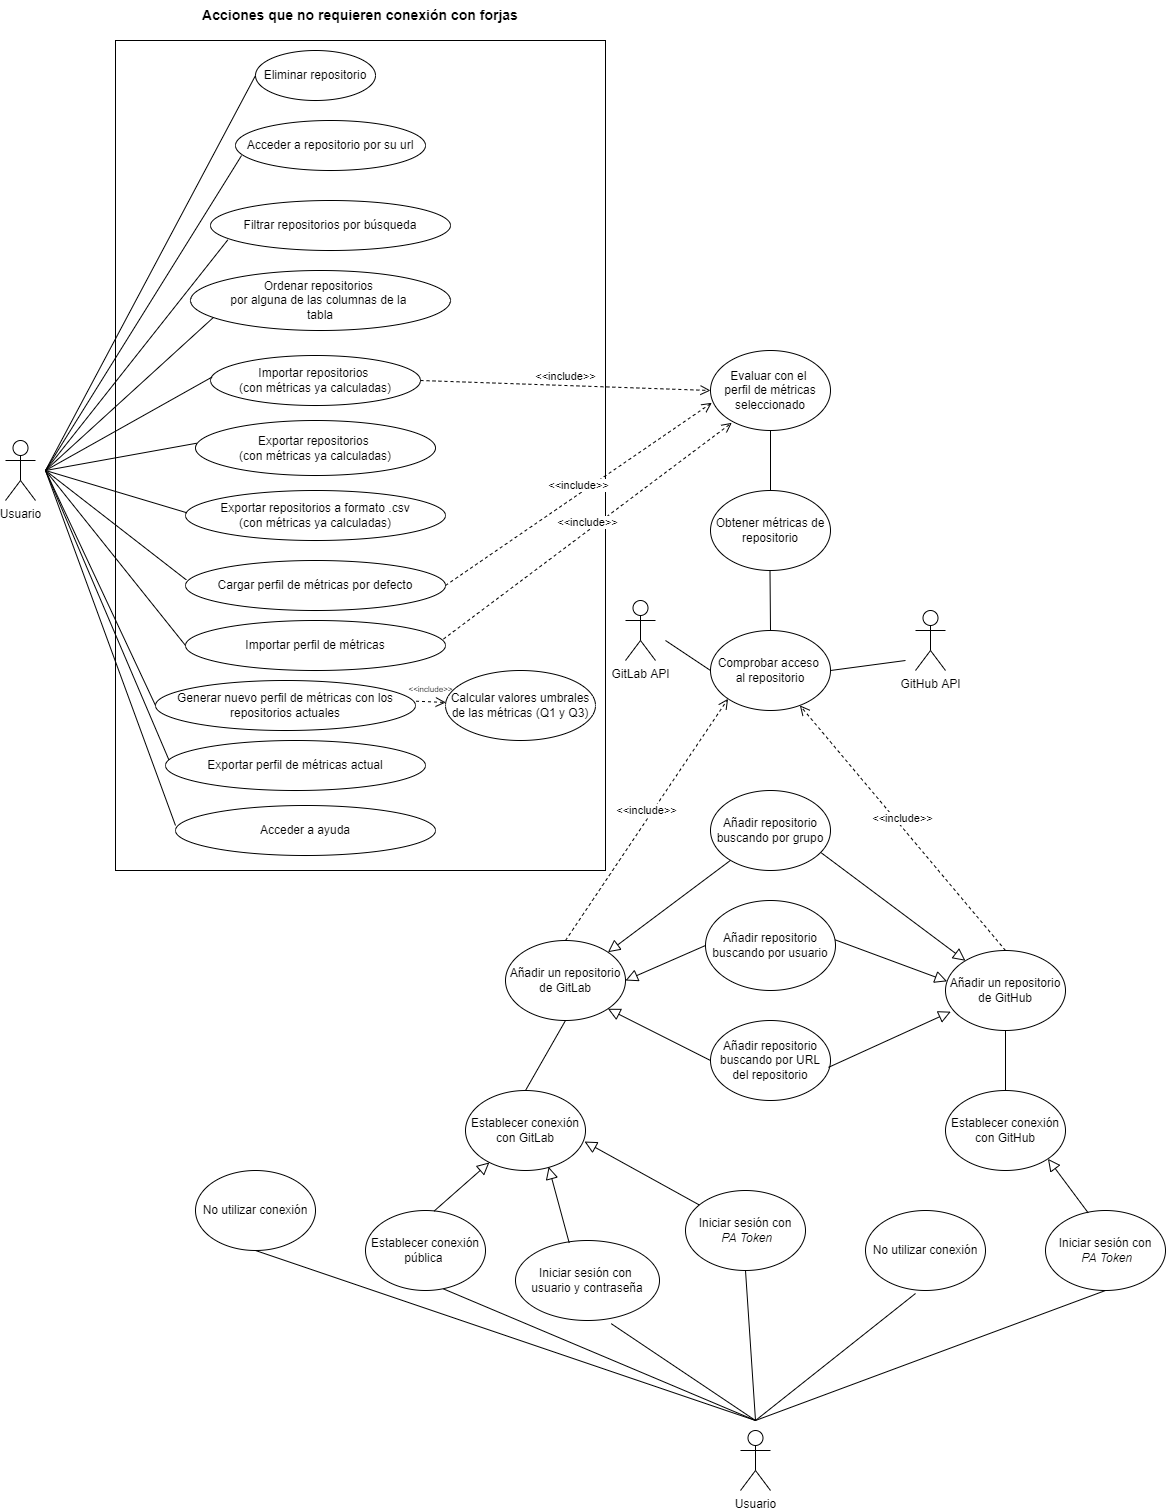
\includegraphics[width=1\textwidth]{AnexC_Use_Cases}
	\caption{Diagrama de casos de uso del proyecto}
	\label{fig:AnexC_Use_Cases}
\end{figure}
\FloatBarrier

A continuación se van a detallar los diferentes casos de uso por medio de tablas \cite{TFMANVIRECO} descriptivas:

\casoDeUso{
	CU-01
}{
	Establecer conexión con \textit{GitHub}
}{
	\tablaCasoDeUso{
		1.0
	}{
		RF-1, RF-1.1, RF-1.2, RF-1.3, RF-1.4
	}{
		Permite al usuario establecer una conexión con \textit{GitHub} para posteriormente poder importar repositorios y calcular sus métricas.
	}{
		Situado en la página principal.
	}{
		1 & Pulsar el botón de conexión con \textit{GitHub}. \\
		2 & Pulsar el botón \textit{Connect} en el diálogo de estado de la conexión. \\
		3 & Rellenar el \textit{input} del \textit{Personal Access Token} y pulsar el botón \textit{Connect} en el diálogo de conexión.
	}{
		Se ha establecido una conexión con \textit{GitHub} que permite importar repositorios de esta forja.
	}{
		1 & No se pulsa el botón \textit{Connect} en el diálogo de estado de la conexión. \\
		2 & Se selecciona el botón \textit{Don't connect} en el diálogo de conexión. \\
		3 & No se introduce un \textit{Personal Access Token} válido.
	}{Alta}{cu-01}
}

\casoDeUso{
	CU-02
}{
	Establecer conexión con \textit{GitLab}
}{
	\tablaCasoDeUso{
		1.0
	}{
		RF-2, RF-2.1, RF-2.2, RF-2.3, RF-2.4, RF-2.5, RF-2.6, RF-2.7
	}{
		Permite al usuario establecer una conexión con \textit{GitLab} para posteriormente poder importar repositorios y calcular sus métricas.
	}{
		Situado en la página principal.
	}{
		1 & Pulsar el botón de conexión con \textit{GitLab}. \\
		2 & Pulsar el botón \textit{Connect} en el diálogo de estado de la conexión. \\
		3.a & Rellenar los \textit{input} del \textit{Username} y \textit{Password} y pulsar el botón \textit{Connect} en el diálogo de conexión.  \\
		3.b & Seleccionar la opción \textit{Personal Access Token}, rellenar el \textit{input} del \textit{Personal Access Token} y pulsar el botón \textit{Connect} en el diálogo de conexión.\\
		3.c & Seleccionar la opción \textit{Public connection} y pulsar el botón \textit{Connect} en el diálogo de conexión.

	}{
		Se ha establecido una conexión con \textit{GitLab} que permite importar repositorios de esta forja.
	}{
		1 & No se pulsa el botón \textit{Connect} en el diálogo de estado de la conexión. \\
		2 & Se selecciona el botón \textit{Don't connect} en el diálogo de conexión. \\
		3.a & No se introducen un usuario y contraseña válidos. \\
		3.b & No se introduce un \textit{Personal Access Token} válido.
	}{Alta}{cu-02}
}

\casoDeUso{
	CU-03
}{
	Añadir un nuevo proyecto
}{
	\tablaCasoDeUso{
		1.0
	}{
		RF-3, RF-3.1, RF-3.1.1, RF-3.1.2, RF-3.1.3, RF-3.2, RF-3.3, RF-4, RF-4.2, RF-4.5, RF-4.6
	}{
		Añadir un nuevo proyecto para calcular sus métricas y evaluarlo.
	}{
		Se ha establecido una conexión.	
	}{
		1 & Pulsar el botón \textit{Project management}. \\
		2.a & Pulsar el botón \textit{Add new GitLab repository} en las opciones del desplegable. \\
		2.b & Pulsar el botón \textit{Add new GitHub repository} en las opciones del desplegable. \\
		3.a & Rellenar el input \textit{User ID or username}, seleccionar uno de los resultados del desplegable \textit{Project}.  \\
		3.b & Seleccionar la opción \textit{By Group}, rellenar el \textit{input} del \textit{Group ID or groupname}, seleccionar uno de los resultados del desplegable \textit{Project}. \\
		3.c & Seleccionar la opción \textit{By URL}, rellenar el input \textit{Project URL}. \\
		4 & Pulsar el botón \textit{Add}. \\
		5 & Se obtiene el proyecto y se calculan las métricas. \\
		6 & Se evalúan las métricas con el perfil de métricas seleccionado actualmente. \\
		7 & Se añade el proyecto al listado.
	}{
		Se ha añadido el proyecto al listado con sus métricas calculadas y evaluadas.
	}{
		1 & No se introducen un  \textit{User ID or username} o \textit{Group ID or groupname} o bien \textit{Project URL} válidos. \\
		2 & La conexión establecida no tiene permisos suficientes para acceder al repositorio solicitado.  \\
		3 & Se intenta añadir un proyecto que ya está añadido previamente.
	}{Alta}{cu-03}
}


\casoDeUso{
	CU-04
}{
	Eliminar un proyecto
}{
	\tablaCasoDeUso{
		1.0
	}{
		RF-3.3
	}{
		Eliminar un proyecto del listado.
	}{
		Existe algún proyecto que eliminar.	
	}{
		1 & Pulsar el botón \textit{papelera} de la fila del listado correspondiente al proyecto que se desea eliminar. \\
		2 & El proyecto es eliminado del listado.
	}{
		El proyecto eliminado ya no está en el listado.
	}{
		1 & Se produce un error al eliminar el repositorio y éste permanece en el listado. 
	}{Baja}{cu-04}
}

\casoDeUso{
	CU-05
}{
	Volver a obtener métricas de un repositorio
}{
	\tablaCasoDeUso{
		1.0
	}{
		RF-3.5
	}{
		Permite volver a obtener las métricas de un repositorio ya añadido al listado.
	}{
		Se ha establecido una conexión a la forja origen del repositorio.
	}{
		1 & Pulsar el botón \textit{libro-calculadora} de la fila del listado correspondiente al proyecto que se desea actualizar. \\
		2 & Las métricas del proyecto son calculadas y evaluadas con el perfil actual. \\
	}{
		Las métricas del proyecto han sido calculadas y evaluadas con el perfil actual.
	}{
		1 & No existe conexión con la forja correspondiente. \\
		2 & La conexión actual no tiene permisos suficientes para obtener las métricas del repositorio.
	}{Baja}{cu-05}
}

\casoDeUso{
	CU-06
}{
	Exportar proyectos y métricas a formato `.emr'
}{
	\tablaCasoDeUso{
		1.0
	}{
		RF-3.6
	}{
		Permite exportar los proyectos y sus métricas ya calculadas en un formato que permite importación.
	}{
		Existen proyectos en el listado.
	}{
		1 & Pulsar el botón \textit{Project management}. \\
		2 & Pulsar el botón \textit{Export} del desplegable. \\
		3 & Pulsar el botón \textit{Download} del diálogo de confirmación. \\
		4 & Los repositorios y sus métricas son exportados en un archivo con formato `.emr'. \\
	}{
		Obtenemos un archivo que contiene la información de los repositorios y sus métricas en formato `.emr'.
	}{
		1 & No existen proyectos en el listado.
	}{Media}{cu-06}
}

\casoDeUso{
	CU-07
}{
	Exportar proyectos y métricas a formato `.csv'
}{
	\tablaCasoDeUso{
		1.0
	}{
		RF-3.7
	}{
		Permite exportar los proyectos y sus métricas ya calculadas en un formato que permite su uso por ejemplo en hojas de cálculo.
	}{
		Existen proyectos en el listado.
	}{
		1 & Pulsar el botón \textit{Project management}. \\
		2 & Pulsar el botón \textit{Export to CSV} del desplegable. \\
		3 & Pulsar el botón \textit{Download} del diálogo de confirmación. \\
		4 & Los repositorios y sus métricas son exportados en un archivo con formato `.csv'. \\
	}{
		Obtenemos un archivo que contiene la información de los repositorios y sus métricas en formato `.csv'.
	}{
		1 & No existen proyectos en el listado.
	}{Media}{cu-07}
}

\casoDeUso{
	CU-08
}{
	Importar proyectos desde archivo.
}{
	\tablaCasoDeUso{
		1.0
	}{
		RF-3.8, RF-3.9
	}{
		Permite importar una lista de proyectos con sus métricas desde un archivo con formato `.emr'.
	}{
		Existen proyectos en el listado.
	}{
		1 & Pulsar el botón \textit{Project management}. \\
		2 & Pulsar el botón \textit{Import} del desplegable. \\
		3.a & Pulsar el botón \textit{Upload File...} del diálogo de importación y seleccionar un archivo en el explorador de archivos. \\
		3.b & Soltar un fichero en la zona \textit{Drop file here}. \\
		4 & Si se detecta que ya hay repositorios con el mismo nombre, elegir si queremos sobreescrirlos o añadir sólo los que no estén. \\
		5 & Los repositorios del fichero y sus métricas son importados al listado y evaluados con el perfil actual. No se importa ningún proyecto que ya exista. \\
	}{
		Los repositorios del fichero y sus métricas son importados al listado y evaluados con el perfil actual, no se tiene ningún proyecto duplicado.
	}{
		1 & No se selecciona un archivo válido.
	}{Media}{cu-08}
}

\casoDeUso{
	CU-09
}{
	Filtrar proyectos.
}{
	\tablaCasoDeUso{
		1.0
	}{
		RF-3.10
	}{
		Permite filtrar los proyectos del listado por su nombre.
	}{
		Existen proyectos en el listado.
	}{
		1 & Escribir en el input \textit{Search} el texto a buscar. \\
		2 & En el listado sólo se mostrarán los proyectos que contengan dicho texto en su nombre.
	}{
		En el listado sólo se muestran los proyectos que contengan el texto buscado en su nombre.
	}{
		1 & No existen proyectos en el listado.	
	}{Baja}{cu-09}
}


\casoDeUso{
	CU-10
}{
	Ordenar proyectos.
}{
	\tablaCasoDeUso{
		1.0
	}{
		RF-3.11, RF-3.12
	}{
		Permite ordenar los proyectos por nombre, fecha o cualquiera de las métricas.
	}{
		Existen proyectos en el listado.
	}{
		1 & Hacer \textit{click} sobre el icono de ordenación de la columna por la que se desea ordenar (ascendente). \\
		2 & Volver a hacer \textit{click} si se desea cambiar a ordenación descendente. \\
		2 & Volver a hacer \textit{click} si se cancelar la ordenación. \\
		4 & Los proyectos de listado aparecen ordenados según la columna y criterio seleccionados.
	}{
		En el listado sólo se muestran los proyectos ordenados por la columna seleccionada y en el orden seleccionado.
	}{
		1 & No existen proyectos en el listado.	
	}{Baja}{cu-10}
}

\casoDeUso{
	CU-11
}{
	Evaluar con nuevo perfil de métricas
}{
	\tablaCasoDeUso{
		1.0
	}{
		RF-4.3
	}{
		Permite generar un perfil de métricas con los proyectos existentes en el listado y evaluarlos con el mismo.
	}{
		Existen proyectos en el listado.
	}{
		1 & Pulsar el botón \textit{Evaluate projects}. \\
		2 & Pulsar el botón \textit{Evaluate with new profile} del desplegable. \\
		3 & Los proyectos del listado son evaluados con el nuevo perfil generado a partir de ellos.
	}{
		Los proyectos del listado han sido evaluados con el nuevo perfil generado a partir de ellos.
	}{
		1 & No existen proyectos en el listado.	
	}{Alta}{cu-11}
}

\casoDeUso{
	CU-12
}{
	Exportar perfil de métricas
}{
	\tablaCasoDeUso{
		1.0
	}{
		RF-4.4
	}{
		Permite exportar el perfil de métricas actual en formato `.emr', éste es importable.
	}{
		Existen proyectos en el listado.
	}{
		1 & Pulsar el botón \textit{Evaluate projects}. \\
		2 & Pulsar el botón \textit{Export actual profile} del desplegable. \\
		3 & Pulsar el botón \textit{Download} del diálogo \textit{Export metric profile}. \\
		4 & El perfil de métricas actual es exportado.
	}{
		Obtenemos un fichero en formato `.emr' que contiene la información del perfil actual de métricas.
	}{
		1 & No existen proyectos en el listado.	
	}{Alta}{cu-12}
}

\casoDeUso{
	CU-13
}{
	Importar perfil de métricas
}{
	\tablaCasoDeUso{
		1.0
	}{
		RF-4.5
	}{
		Permite importar un perfil de métricas desde un archivo en formato `.emr'.
	}{
		Existen proyectos en el listado.
	}{
		1 & Pulsar el botón \textit{Evaluate projects}. \\
		2 & Pulsar el botón \textit{Evaluate with imported profile} del desplegable. \\
		3.a & Pulsar el botón \textit{Upload File...} del diálogo de importación y seleccionar un archivo en el explorador de archivos. \\
		3.b & Soltar un fichero en la zona \textit{Drop file here}. \\
		4 & El perfil de métricas es importado y los proyectos son evaluados con el.
	}{
		Se ha cargado un nuevo perfil de métricas y los proyectos del listado son evaluados con él.
	}{
		1 & No se ha seleccionado un archivo válido	
	}{Alta}{cu-13}
}